% ============================================================================
% CHAPTER 3: CASE STUDY
% ============================================================================
\chapter{Case Study: Office Building Scenario}
\label{ch:case_study}

This chapter describes the specific office building scenario used to evaluate the smart charging algorithms. We present the data sources, parameter selection, and justification for the chosen values.

\section{Overview}
\label{sec:case_study_overview}

The case study simulates a typical office building with:
\begin{itemize}
    \item Rooftop solar PV installation
    \item Workplace EV charging infrastructure for 15 vehicles
    \item Grid connection with capacity constraints
    \item 24-hour simulation period on a representative workday
\end{itemize}

\section{Building Energy Profile}
\label{sec:building_profile}

\subsection{Energy Consumption Data}
\label{subsec:consumption_data}

\subsubsection{Data Source}

The building energy consumption profile is derived from the ELMAS (European Load Model for Aggregated Sectors) dataset, specifically the Office cluster (\#5):
\begin{itemize}
    \item Dataset: \texttt{office\_single\_building\_timeseries.csv}
    \item Source: ELMAS dataset -- \texttt{Time\_series\_18\_clusters.csv} (Office cluster \#5)
    \item Building type: Office/commercial
    \item Target annual energy: 58,831~kWh (75th percentile of per-customer distribution)
    \item Temporal resolution: Hourly (8,736 data points for year 2018)
\end{itemize}

The profile was constructed by scaling the cluster load shape to a single-building target energy and adding stochastic variability (daily $\sigma_d = 0.08$, hourly $\sigma_h = 0.03$) to introduce realistic fluctuations, followed by re-normalization to preserve the annual energy total (see Section~\ref{subsec:building_model} for full methodology).

\subsubsection{Profile Characteristics}

Figure \ref{fig:building_consumption} shows the hourly consumption pattern:

\begin{figure}[H]
    \centering
    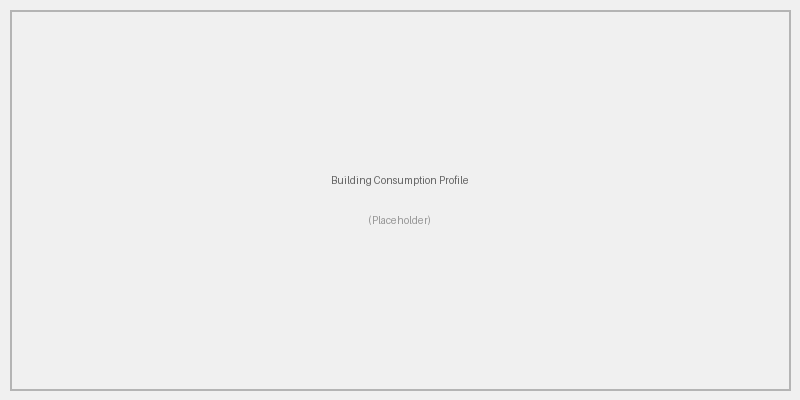
\includegraphics[width=0.8\textwidth]{figures/building_consumption_profile.png}
    \caption{Office building hourly energy consumption profile}
    \label{fig:building_consumption}
\end{figure}

Key characteristics:
\begin{itemize}
    \item Mean load: 6.73~kW
    \item Peak load: 11.92~kW (business hours)
    \item Annual energy: 58,831~kWh
    \item Daily consumption: $\sim$161~kWh (annual / 365)
\end{itemize}

\subsubsection{Validation}

The consumption profile is validated against the ELMAS source data:
\begin{itemize}
    \item The per-customer annual energy distribution (mean 10,429~kWh, P75 = 58,831~kWh) spans small to large office buildings
    \item The 75th percentile was chosen to represent a medium-to-large office
    \item The cluster load shape preserves realistic hourly patterns (working-hours peak, overnight baseline)
    \item Stochastic noise ensures the profile is not artificially smooth while preserving the correct total energy
\end{itemize}

\subsection{Solar PV System}
\label{subsec:solar_system}

\subsubsection{System Specifications}

The rooftop solar PV system parameters:

\begin{table}[H]
\centering
\caption{Solar PV system specifications}
\label{tab:pv_specs}
\begin{tabular}{@{}ll@{}}
\toprule
\textbf{Parameter} & \textbf{Value} \\
\midrule
Panel area & 150 m² \\
Panel efficiency & 20\% \\
Peak power & 30 kW \\
Technology & [e.g., Monocrystalline silicon] \\
\bottomrule
\end{tabular}
\end{table}

\subsubsection{Irradiance Data}

Solar irradiance data is obtained from PVGIS (Photovoltaic Geographical Information System):

\begin{itemize}
    \item Source: European Commission Joint Research Centre PVGIS database
    \item Location: [Specify coordinates/city]
    \item Date: March 12, 2018 (representative spring day)
    \item Temporal resolution: Hourly
    \item Data file: \texttt{irradiance\_pvgis.csv}
\end{itemize}

\subsubsection{Solar Production Profile}

The hourly solar power production:

\begin{equation}
P_{solar}(t) = A_{panel} \cdot \eta_{panel} \cdot I(t) = 150 \, \text{m}^2 \cdot 0.20 \cdot I(t)
\end{equation}

Figure \ref{fig:solar_profile} illustrates the production profile:

\begin{figure}[H]
    \centering
    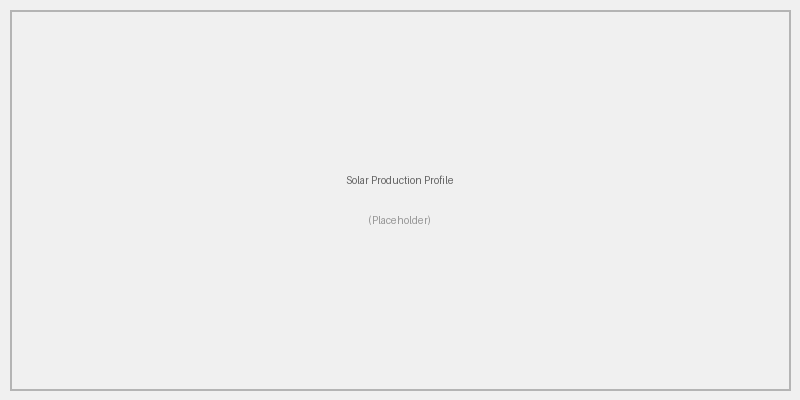
\includegraphics[width=0.8\textwidth]{figures/solar_production_profile.png}
    \caption{Hourly solar PV production profile (March 12, 2018)}
    \label{fig:solar_profile}
\end{figure}

Key observations:
\begin{itemize}
    \item Peak production: $\sim$[X] kW at solar noon (12-2 PM)
    \item Total daily production: [Calculate] kWh
    \item Production exceeds building consumption during midday hours
    \item Temporal alignment with EV parking hours (6 AM - 6 PM)
\end{itemize}

\subsubsection{Selection Justification}

March 12, 2018 was selected because:
\begin{itemize}
    \item Representative spring day (moderate solar production)
    \item Clear sky conditions (good for demonstrating solar benefits)
    \item Typical seasonal pattern (not extreme summer/winter)
    \item Available validated data from PVGIS
\end{itemize}

\subsection{Building Battery Storage}
\label{subsec:building_battery}

The building includes a stationary battery storage system:

\begin{table}[H]
\centering
\caption{Building battery specifications}
\label{tab:building_battery}
\begin{tabular}{@{}ll@{}}
\toprule
\textbf{Parameter} & \textbf{Value} \\
\midrule
Capacity & 80 kWh \\
Efficiency & 95\% \\
Initial SoC & 50\% \\
Depth of discharge limit & 80\% \\
Max charge rate & 50 kW \\
Max discharge rate & 50 kW \\
\bottomrule
\end{tabular}
\end{table}

\section{Electric Vehicle Fleet}
\label{sec:ev_fleet}

\subsection{Fleet Composition}
\label{subsec:fleet_composition}

The simulation considers a fleet of 15 electric vehicles, representing a typical office building with 50-100 employees (assuming 15-30\% EV adoption).

\subsubsection{Vehicle Specifications}

Each EV is modeled with identical technical characteristics:

\begin{table}[H]
\centering
\caption{Electric vehicle specifications}
\label{tab:ev_specs}
\begin{tabular}{@{}ll@{}}
\toprule
\textbf{Parameter} & \textbf{Value} \\
\midrule
Battery capacity & 100 kWh \\
Reference vehicle & Tesla Model 3 Long Range \\
Max charge rate & 22 kW (Level 2 AC charger) \\
Max discharge rate & 22 kW (V2G capable) \\
Energy consumption & 0.18 kWh/km \\
Depth of discharge limit & 90\% \\
Minimum SoC & 20\% \\
\bottomrule
\end{tabular}
\end{table}

\subsubsection{Justification}

\begin{itemize}
    \item \textbf{100 kWh capacity:} Representative of modern long-range EVs (Tesla Model 3, Hyundai Ioniq 5, etc.)
    \item \textbf{22 kW charging:} Standard Level 2 AC charging (common in workplace installations)
    \item \textbf{0.18 kWh/km:} Typical energy consumption for mid-size EVs
    \item \textbf{20\% minimum SoC:} Prevents deep discharge and battery degradation
\end{itemize}

\subsection{Mobility Patterns}
\label{subsec:mobility_patterns}

\subsubsection{Arrival and Departure Times}

The EV fleet follows typical office worker patterns:

\begin{table}[H]
\centering
\caption{EV mobility parameters}
\label{tab:mobility}
\begin{tabular}{@{}ll@{}}
\toprule
\textbf{Parameter} & \textbf{Value} \\
\midrule
Arrival window & 6:00 - 9:00 AM \\
Departure window & 4:00 - 8:00 PM \\
Parking duration & 7-14 hours \\
Initial SoC range & 20-30\% \\
Desired SoC range & 70-80\% \\
\bottomrule
\end{tabular}
\end{table}

Each EV's specific arrival and departure times are randomly sampled from the specified windows to simulate realistic variability.

\subsubsection{State of Charge Requirements}

\begin{itemize}
    \item \textbf{Initial SoC (20-30\%):} Represents battery level after morning commute (assuming 30-50 km commute)
    \item \textbf{Desired SoC (70-80\%):} Ensures sufficient charge for evening commute plus reserve (100-150 km range)
\end{itemize}

\subsubsection{Justification}

The mobility pattern reflects typical office workers:
\begin{itemize}
    \item Morning arrival spread (6-9 AM) accounts for flexible work hours
    \item Evening departure spread (4-8 PM) reflects varied work schedules
    \item Long parking duration provides flexibility for smart charging
    \item SoC requirements ensure mobility needs are met
\end{itemize}

\section{Grid Parameters}
\label{sec:grid_parameters}

\subsection{Electricity Pricing}
\label{subsec:pricing}

\subsubsection{Time-of-Use Tariff}

The simulation uses a realistic time-of-use (TOU) pricing structure:

\begin{figure}[H]
    \centering
    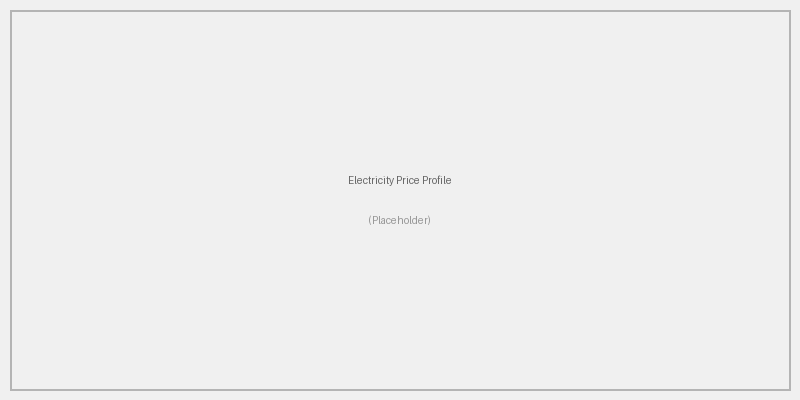
\includegraphics[width=0.9\textwidth]{figures/electricity_price_profile.png}
    \caption{Hourly electricity purchase and sell-back prices}
    \label{fig:price_profile}
\end{figure}

\begin{table}[H]
\centering
\caption{Electricity price ranges by time period}
\label{tab:prices}
\begin{tabular}{@{}lcc@{}}
\toprule
\textbf{Time Period} & \textbf{Purchase Price (€/kWh)} & \textbf{Sell Price (€/kWh)} \\
\midrule
Night (00:00-03:00) & 0.48 & 0.38 \\
Early morning (04:00-07:00) & 0.58-0.70 & 0.48-0.60 \\
Morning (08:00-11:00) & 0.35-0.50 & 0.25-0.40 \\
Midday (12:00-15:00) & 0.18-0.30 & 0.10-0.20 \\
Evening peak (16:00-19:00) & 0.25-0.55 & 0.20-0.50 \\
Night (20:00-23:00) & 0.30-0.50 & 0.25-0.45 \\
\bottomrule
\end{tabular}
\end{table}

\subsubsection{Price Profile Justification}

The pricing structure reflects real-world patterns:
\begin{itemize}
    \item \textbf{Morning peak (4-7 AM):} High demand as buildings start operations
    \item \textbf{Midday low (12-3 PM):} Abundant solar generation reduces grid prices
    \item \textbf{Evening peak (4-7 PM):} High demand as solar production decreases
    \item \textbf{Sell-back prices:} Typically 80-90\% of purchase prices (realistic for feed-in tariffs)
\end{itemize}

Data source: [Cite electricity market data, utility tariffs, or similar studies]

\subsection{Grid Capacity Constraints}
\label{subsec:grid_capacity}

\subsubsection{Capacity Limits}

The grid connection has hourly capacity limits:

\begin{equation}
P_{grid,max}(t) = 80 \, \kw \quad \forall t
\end{equation}

\subsubsection{Justification}

The 80 kW limit represents:
\begin{itemize}
    \item Typical distribution transformer capacity for small commercial buildings
    \item Building baseline consumption: $\sim$8 kW
    \item Available for EV charging: $\sim$70 kW (sufficient for 3-4 simultaneous Level 2 chargers)
    \item Creates realistic constraint requiring intelligent coordination
\end{itemize}

Without smart charging, 15 EVs at 22 kW each would require 330 kW, far exceeding the 80 kW limit. This constraint necessitates intelligent scheduling.

\section{Simulation Configuration}
\label{sec:simulation_config}

\subsection{Time Parameters}
\label{subsec:time_params}

\begin{table}[H]
\centering
\caption{Simulation time parameters}
\label{tab:time_params}
\begin{tabular}{@{}ll@{}}
\toprule
\textbf{Parameter} & \textbf{Value} \\
\midrule
Simulation duration & 24 hours \\
Time step & 1 hour \\
Simulation date & March 12, 2018 \\
Start time & 00:00 (midnight) \\
End time & 23:00 (11 PM) \\
\bottomrule
\end{tabular}
\end{table}

\subsection{Algorithm Parameters}
\label{subsec:algorithm_params}

Each optimization algorithm requires specific hyperparameters:

\subsubsection{Reinforcement Learning}

\begin{table}[H]
\centering
\caption{Q-Learning hyperparameters}
\label{tab:rl_params}
\begin{tabular}{@{}lll@{}}
\toprule
\textbf{Parameter} & \textbf{Charge-Only} & \textbf{V2G} \\
\midrule
Training episodes & 8,000 & 15,000 \\
Learning rate ($\alpha$) & 0.15 & 0.15 \\
Discount factor ($\gamma$) & 0.99 & 1.0 \\
Exploration rate ($\epsilon$) & 0.35 & 0.10 \\
SoC discretization & 0.1 (10\% bins) & 0.1 (10\% bins) \\
\bottomrule
\end{tabular}
\end{table}

Justification:
\begin{itemize}
    \item Higher episodes for V2G due to increased complexity (3 actions vs 2)
    \item $\gamma = 1.0$ for V2G: Future rewards equally important (long-term planning)
    \item Lower $\epsilon$ for V2G: More exploitation after learning optimal policy
\end{itemize}


\section{Data Sources Summary}
\label{sec:data_sources}

\begin{table}[H]
\centering
\caption{Summary of data sources}
\label{tab:data_sources}
\begin{tabular}{@{}lll@{}}
\toprule
\textbf{Data Type} & \textbf{Source} & \textbf{Reference} \\
\midrule
Building consumption & ELMAS dataset (Office cluster \#5) & \cite{elmas} \\
Solar irradiance & PVGIS & \cite{pvgis} \\
Electricity prices & Time-of-use tariff & \cite{electricity_prices} \\
EV specifications & Tesla Model 3 & \cite{tesla_specs} \\
Charging standards & IEC 61851 & \cite{iec61851} \\
\bottomrule
\end{tabular}
\end{table}

\section{Simulation Scenarios}
\label{sec:scenarios}

\subsection{Scenario 1: Charge-Only (No V2G)}
\label{subsec:scenario_charge_only}

\textbf{Configuration:} \texttt{multi\_ev\_config.yml}

This scenario evaluates unidirectional charging with:
\begin{itemize}
    \item 15 EVs with charge-only capability
    \item Algorithms: Simple, RL (Q-Learning)
    \item Grid capacity: 80 kW
    \item No discharge allowed
\end{itemize}

\textbf{Purpose:} Establish baseline performance for intelligent charging without V2G.

\subsection{Scenario 2: V2G-Enabled}
\label{subsec:scenario_v2g}

\textbf{Configuration:} \texttt{multi\_ev\_v2g\_config.yml}

This scenario adds bidirectional capability:
\begin{itemize}
    \item Same 15 EVs with V2G capability
    \item Algorithms: Simple, RL (with discharge action)
    \item Sell-back prices: 80-90\% of purchase prices
    \item Discharge constraints: Preserve desired SoC
\end{itemize}

\textbf{Purpose:} Quantify additional benefits of V2G technology.

\section{Evaluation Metrics}
\label{sec:metrics}

The following metrics are used to evaluate each approach:

\subsection{Economic Metrics}

\begin{itemize}
    \item \textbf{Total Daily Cost:} Sum of electricity purchases minus V2G revenue (€)
    \item \textbf{Cost per kWh:} Average cost per kWh charged (€/kWh)
    \item \textbf{Savings vs Baseline:} Percentage cost reduction compared to Level 0 (\%)
\end{itemize}

\subsection{Energy Metrics}

\begin{itemize}
    \item \textbf{Total Grid Consumption:} Energy purchased from grid (kWh)
    \item \textbf{Renewable Utilization:} Percentage of charging from solar (%)
    \item \textbf{V2G Energy:} Total energy discharged back to grid (kWh, V2G only)
\end{itemize}

\subsection{Performance Metrics}

\begin{itemize}
    \item \textbf{Target Achievement:} Percentage of EVs reaching desired SoC (\%)
    \item \textbf{Average Final SoC:} Mean SoC across fleet at departure time (\%)
    \item \textbf{Grid Violations:} Number of hours exceeding grid capacity
    \item \textbf{SoC Violations:} Number of instances below minimum SoC
\end{itemize}

\subsection{Computational Metrics}

\begin{itemize}
    \item \textbf{Execution Time:} Computation time per simulation (seconds)
    \item \textbf{Training Time:} Time required for learning-based methods (seconds)
    \item \textbf{Scalability:} Performance with varying fleet sizes
\end{itemize}

\section{Implementation}
\label{sec:implementation}

\subsection{Software Environment}

The simulation is implemented in Python 3.x with the following libraries:

\begin{table}[H]
\centering
\caption{Software dependencies}
\label{tab:software}
\begin{tabular}{@{}ll@{}}
\toprule
\textbf{Library} & \textbf{Purpose} \\
\midrule
NumPy & Numerical computations \\
Matplotlib & Visualization \\
PyYAML & Configuration management \\
\bottomrule
\end{tabular}
\end{table}

\subsection{Code Structure}

The implementation follows object-oriented design:

\begin{lstlisting}[language=Python,caption={Main simulation components}]
# Core models
- Building: Energy consumption, solar production, battery
- ElectricVehicle: Battery dynamics, charging/discharging
- Grid: Pricing, capacity constraints

# Charging systems
- MultiEVChargingSystem: Charge-only algorithms
- MultiEVV2GChargingSystem: V2G-enabled algorithms

# Simulation orchestration
- multi_ev_simulator: Run charge-only scenarios
- multi_ev_v2g_simulator: Run V2G scenarios
\end{lstlisting}

\section{Summary}
\label{sec:case_study_summary}

This chapter described the office building case study used to evaluate smart charging algorithms. The scenario includes:
\begin{itemize}
    \item Realistic building energy profile from validated data sources
    \item Solar PV system with PVGIS irradiance data
    \item Fleet of 15 EVs with typical office worker mobility patterns
    \item Time-of-use electricity pricing and grid capacity constraints
\end{itemize}

The next chapter presents the simulation results and comparative analysis across all intelligence levels.
